\documentclass[a4paper,landscape]{article}
\usepackage[margin=1.0cm]{geometry}
\usepackage{tikz}
\usetikzlibrary{positioning, arrows.meta, shapes, shapes.geometric, fit, backgrounds, calc}
\usepackage{xcolor}

\definecolor{navy}{RGB}{15,55,130}
\definecolor{steelblue}{RGB}{50,100,180}
\definecolor{skyblue}{RGB}{200,220,255}
\definecolor{teal}{RGB}{0,120,110}
\definecolor{tealfill}{RGB}{200,240,235}
\definecolor{amber}{RGB}{155,85,0}
\definecolor{amberfill}{RGB}{255,235,195}
\definecolor{violet}{RGB}{100,30,150}
\definecolor{violetfill}{RGB}{235,215,255}
\definecolor{layerbg}{RGB}{245,248,255}
\definecolor{layerbdr}{RGB}{150,175,225}
\definecolor{arrcol}{RGB}{60,80,120}
\definecolor{red2}{RGB}{175,30,30}
\definecolor{redfill}{RGB}{255,215,215}

\tikzset{
  CO/.style={draw=steelblue,fill=skyblue,thick,rectangle,minimum width=3.2cm,minimum height=0.9cm,font=\scriptsize\bfseries\sffamily\color{navy},align=center,rounded corners=3pt,inner sep=3pt},
  TC/.style={draw=teal,fill=tealfill,thick,rectangle,minimum width=3.2cm,minimum height=0.9cm,font=\scriptsize\bfseries\sffamily\color{teal},align=center,rounded corners=3pt,inner sep=3pt},
  AC/.style={draw=amber,fill=amberfill,thick,rectangle,minimum width=3.2cm,minimum height=0.9cm,font=\scriptsize\bfseries\sffamily\color{amber},align=center,rounded corners=3pt,inner sep=3pt},
  VC/.style={draw=violet,fill=violetfill,thick,rectangle,minimum width=3.2cm,minimum height=0.9cm,font=\scriptsize\bfseries\sffamily\color{violet},align=center,rounded corners=3pt,inner sep=3pt},
  RC/.style={draw=red2,fill=redfill,thick,rectangle,minimum width=3.2cm,minimum height=0.9cm,font=\scriptsize\bfseries\sffamily\color{red2},align=center,rounded corners=3pt,inner sep=3pt},
  LY/.style={draw=layerbdr,fill=layerbg,thick,rounded corners=5pt,inner sep=6pt},
  FL/.style={->,>=Latex,thick,arrcol},
  RF/.style={->,>=Latex,dashed,thick,red2},
  lb/.style={font=\tiny\sffamily,fill=white,inner sep=0.8pt},
}

\begin{document}
\pagestyle{empty}

\begin{center}
  {\Large\bfseries\sffamily\color{navy} Architecture Diagram --- Metamorphic Circuit Breaker Framework}\\[3pt]
  {\small\sffamily\color{gray} Metamorphic Circuit Breaker: A Runtime Reliability Layer for Detecting Transform-Brittleness in Deployed Vision Models}
\end{center}
\vspace{4pt}

\begin{center}
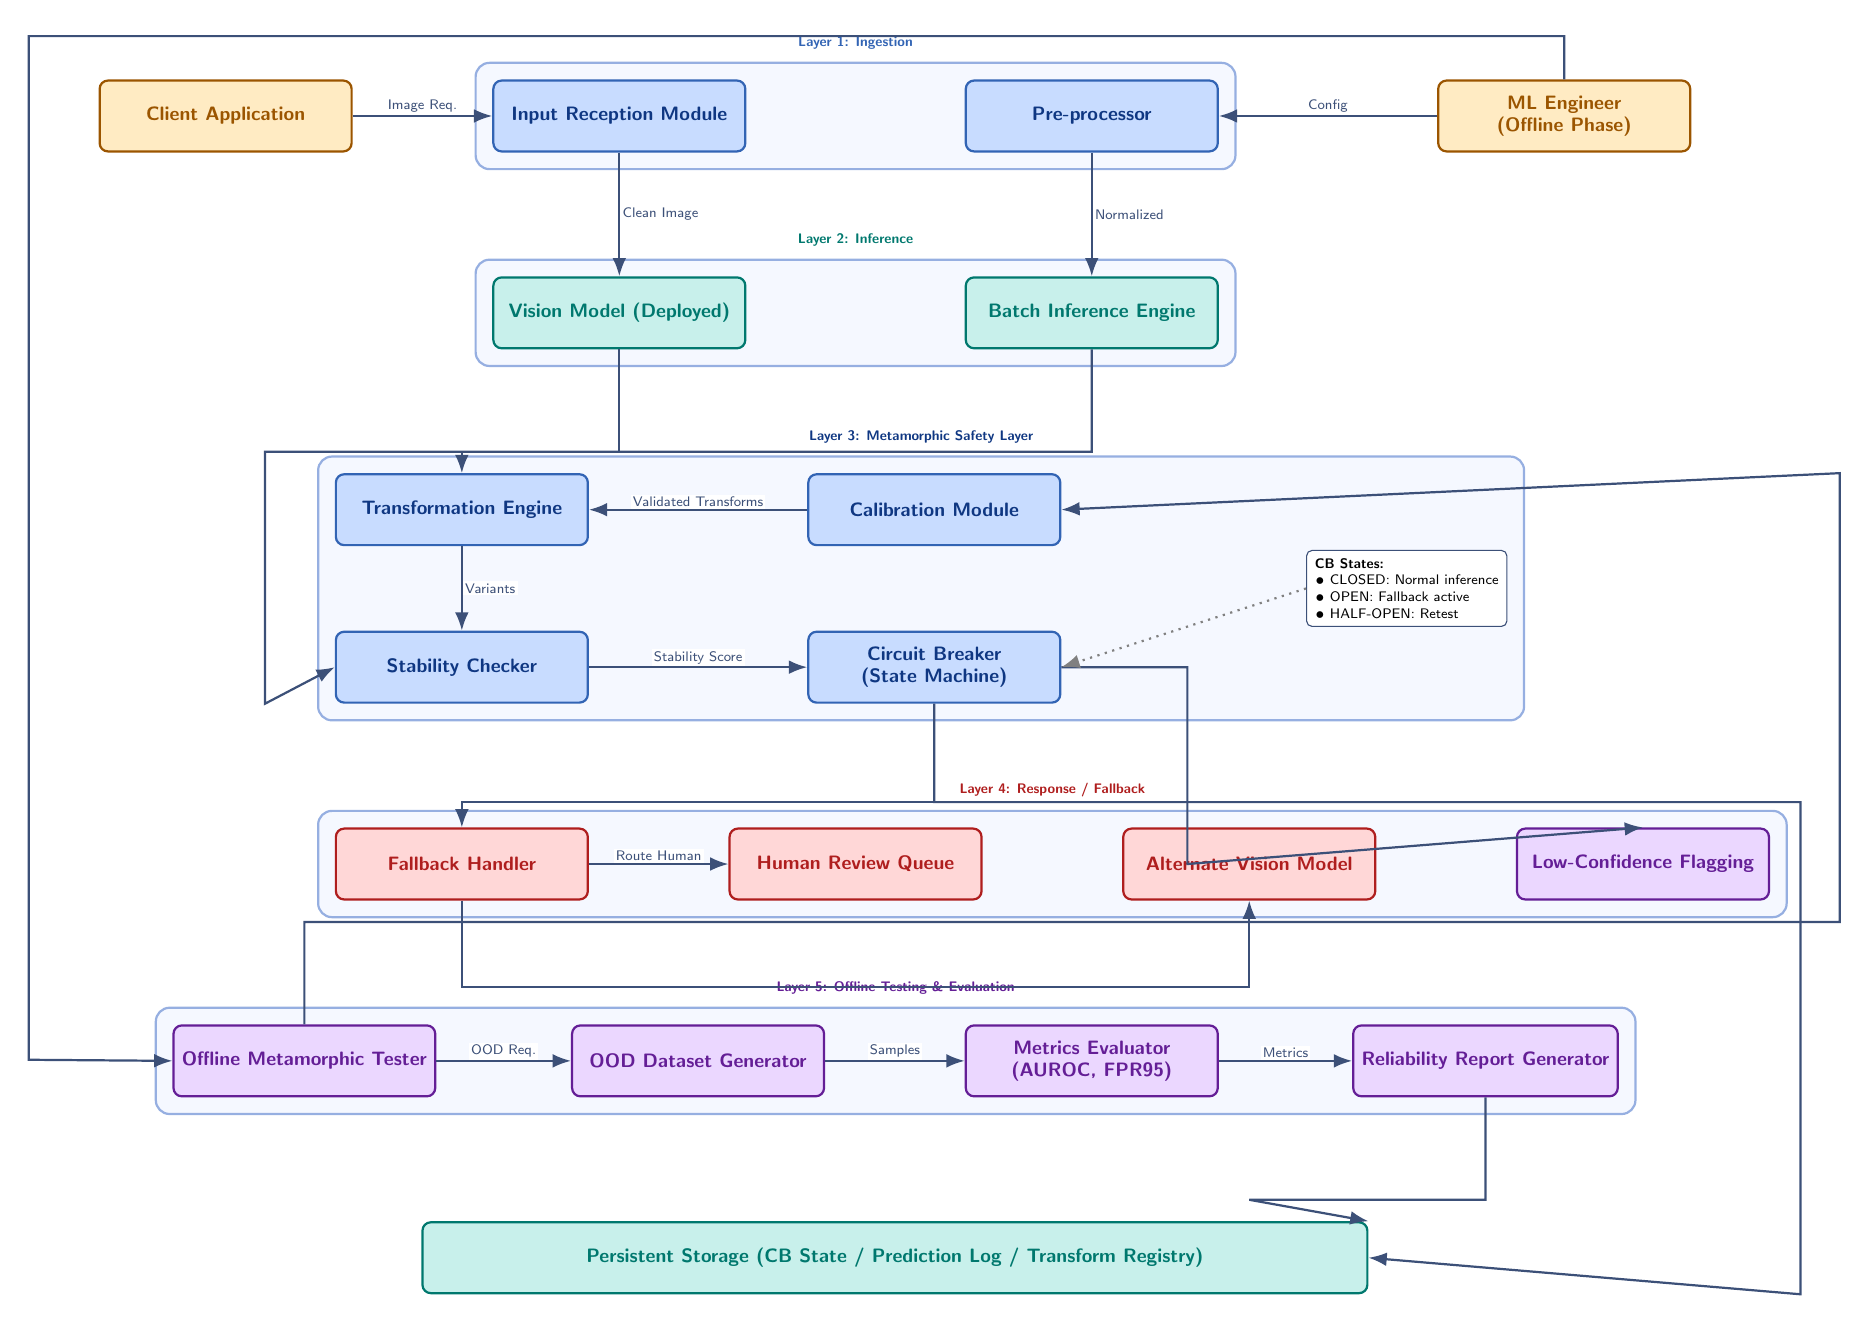
\begin{tikzpicture}[font=\scriptsize\sffamily]

% External / Top
\node[AC](client) at (2.0, 5.0){Client Application};
\node[AC](mleng)  at (19.0, 5.0){ML Engineer\\(Offline Phase)};

% Layer 1: Ingestion (y=5.0)
\node[CO](ingest)  at (7.0, 5.0){Input Reception Module};
\node[CO](preproc) at (13.0, 5.0){Pre-processor};
\begin{pgfonlayer}{background}
  \node[LY,fit=(ingest)(preproc),label={[font=\tiny\bfseries\sffamily\color{steelblue},yshift=1pt]above:Layer 1: Ingestion}](l1){};
\end{pgfonlayer}

% Layer 2: Inference (y=2.5)
\node[TC](vision) at (7.0, 2.5){Vision Model (Deployed)};
\node[TC](batch)  at (13.0, 2.5){Batch Inference Engine};
\begin{pgfonlayer}{background}
  \node[LY,fit=(vision)(batch),label={[font=\tiny\bfseries\sffamily\color{teal},yshift=1pt]above:Layer 2: Inference}](l2){};
\end{pgfonlayer}

% Layer 3: Metamorphic Safety (y=0.0 & -2.0)
\node[CO](te)  at (5.0, 0.0){Transformation Engine};
\node[CO](cal) at (11.0, 0.0){Calibration Module};
\node[CO](sc)  at (5.0,-2.0){Stability Checker};
\node[CO](cb)  at (11.0,-2.0){Circuit Breaker\\(State Machine)};
\node[draw=arrcol,fill=white,rounded corners=2pt,font=\tiny\sffamily,align=left,inner sep=3pt] (cbbox) at (17.0,-1.0){%
  \textbf{CB States:}\\
  $\bullet$ CLOSED: Normal inference\\
  $\bullet$ OPEN: Fallback active\\
  $\bullet$ HALF-OPEN: Retest};
\begin{pgfonlayer}{background}
  \node[LY,fit=(te)(cal)(sc)(cb)(cbbox),label={[font=\tiny\bfseries\sffamily\color{navy},yshift=1pt]above:Layer 3: Metamorphic Safety Layer}](l3){};
\end{pgfonlayer}

% Layer 4: Response (y=-4.5)
\node[RC](fallback) at (5.0,-4.5){Fallback Handler};
\node[RC](human)    at (10.0,-4.5){Human Review Queue};
\node[RC](fbmod)    at (15.0,-4.5){Alternate Vision Model};
\node[VC](lowconf)  at (20.0,-4.5){Low-Confidence Flagging};
\begin{pgfonlayer}{background}
  \node[LY,fit=(fallback)(human)(fbmod)(lowconf),label={[font=\tiny\bfseries\sffamily\color{red2},yshift=1pt]above:Layer 4: Response / Fallback}](l4){};
\end{pgfonlayer}

% Layer 5: Offline (y=-7.0)
\node[VC](offtest) at ( 3.0,-7.0){Offline Metamorphic Tester};
\node[VC](oodgen)  at ( 8.0,-7.0){OOD Dataset Generator};
\node[VC](meteval) at (13.0,-7.0){Metrics Evaluator\\(AUROC, FPR95)};
\node[VC](report)  at (18.0,-7.0){Reliability Report Generator};
\begin{pgfonlayer}{background}
  \node[LY,fit=(offtest)(oodgen)(meteval)(report),label={[font=\tiny\bfseries\sffamily\color{violet},yshift=1pt]above:Layer 5: Offline Testing \& Evaluation}](l5){};
\end{pgfonlayer}

% Storage (y=-9.5)
\node[TC,minimum width=12.0cm](store) at (10.5,-9.5){Persistent Storage (CB State / Prediction Log / Transform Registry)};

% FLOWS
\draw[FL](client.east)--node[lb,above]{Image Req.}(ingest.west);
\draw[FL](mleng.west)--node[lb,above]{Config}(preproc.east);

\draw[FL](ingest.south)--node[lb,right]{Clean Image}(vision.north);
\draw[FL](preproc.south)--node[lb,right]{Normalized}(batch.north);

\draw[FL](vision.south)--++(0,-1.3)--++(-2.0,0)--(te.north);
\draw[FL](batch.south)--++(0,-1.3)--++(-10.5,0)--++(0,-3.2)--(sc.west);

\draw[FL](cal.west)--node[lb,above]{Validated Transforms}(te.east);
\draw[FL](te.south)--node[lb,right]{Variants}(sc.north);
\draw[FL](sc.east)--node[lb,above]{Stability Score}(cb.west);

\draw[FL](cb.south)--++(0,-1.25)--++(-6.0,0)--(fallback.north);
\draw[FL](fallback.east)--node[lb,above]{Route Human}(human.west);
\draw[FL](fallback.south)--++(0,-1.1)--++(10.0,0)--(fbmod.south);

\draw[FL](cb.east)--++(1.6,0)--++(0,-2.5)--(lowconf.north);

\draw[FL](mleng.north)--++(0,0.55)--++(-19.5,0)--++(0,-13.0)--(offtest.west);

% offtest -> cal: routed around far right x=22.5
\draw[FL](offtest.north)--++(0,1.3)--++(19.5,0)--++(0,5.7)--(cal.east);

\draw[FL](offtest.east)--node[lb,above]{OOD Req.}(oodgen.west);
\draw[FL](oodgen.east)--node[lb,above]{Samples}(meteval.west);
\draw[FL](meteval.east)--node[lb,above]{Metrics}(report.west);

\draw[FL](report.south)--++(0,-1.3)--++(-3.0,0)--(store.north east);

% cb -> store: routed down far right x=22.0
\draw[FL](cb.south)--++(0,-1.25)--++(11.0,0)--++(0,-6.25)--(store.east);

\draw[->,>=Latex,dotted,gray,thick](cbbox.west)--(cb.east);

\end{tikzpicture}
\end{center}

\end{document}
